%-----------------------------------------------------------------------------
%
%               Template for sigplanconf LaTeX Class
%
% Name:         sigplanconf-template.tex
%
% Purpose:      A template for sigplanconf.cls, which is a LaTeX 2e class
%               file for SIGPLAN conference proceedings.
%
% Guide:        Refer to "Author's Guide to the ACM SIGPLAN Class,"
%               sigplanconf-guide.pdf
%
% Author:       Paul C. Anagnostopoulos
%               Windfall Software
%               978 371-2316
%               paul@windfall.com
%
% Created:      15 February 2005
%
%-----------------------------------------------------------------------------


\documentclass{sigplanconf}

% The following \documentclass options may be useful:
%
% 10pt          To set in 10-point type instead of 9-point.
% 11pt          To set in 11-point type instead of 9-point.
% authoryear    To obtain author/year citation style instead of numeric.

\usepackage{amsmath}
\usepackage[pdftex]{graphicx}
\usepackage{listings}

\lstset{
basicstyle=\ttfamily,
numberstyle=\small,
commentstyle=\textit
stepnumber=1
}

\begin{document}

\conferenceinfo{CSCI5525 '11}{2011-Dec-15, Boulder, CO.} 
\copyrightyear{2011} 
\copyrightdata{[to be supplied]} 

\titlebanner{banner above paper title}        % These are ignored unless
\preprintfooter{short description of paper}   % 'preprint' option specified.

\title{An Implementation of Reference Counting for a Python to x86 Compiler}
%\subtitle{With Reference Counting Garbage Collection}

\authorinfo{Brent Smith}
           {University of Colorado, Boulder}
           {brent.m.smith@colorado.edu}
\authorinfo{Robert Elsner}
           {University of Colorado, Boulder}
           {robert.elsner@colorado.edu}

\maketitle

\begin{abstract}
Garbage collection in high level languages has enabled increased programmer productivity, but at the cost of performance and ease of implementation for the language designer.  This paper will explore these trade-offs through an implementation of automatic garbage collection for a subset of the Python language.   Our implementation will extend an existing Python to x86 compiler to use reference counting garbage collection.  Reference counting is chosen for its ease of implementation, and because it is less invasive when one of the design goals is to integrate with assembly or C routines without extra intervention from the software developer.  We outline the changes to the existing compiler to enable reference counting, including how the abstract syntax tree of the program is altered, and then discuss the implications of our design choices.
\end{abstract}

\category{D.1.5}{Programming Techniques}{Object-oriented Programming}
\category{D.3.3}{Programming Languages}{Language Constructs And Features-Dynamic Storage Management}
\category{D.3.4}{Programming Languages}{Processors- Memory Management (garbage collection)}
\category{D.4.2}{Operating Systems}{Storage Management-Garbage collection}

\terms
Management, Performance, Design, Languages, Algorithms

\keywords
memory management, garbage collection, reference counting, compilation, compilers, programming languages

\section{Introduction}

Python is a modern, high level language that uses dynamic typing and is run within an interpreter.  It manages memory for the programmer, and is considered by many to be a good ``prototyping'' language, in which programmers can quickly and easily develop an application.   Automatic memory management plays a large part in supporting this role, as it relieves the programmer from the tedious task of remembering when to deallocate memory.  For language designers, deciding what form of memory management to incorporate into their language can be a difficult task.  The choice will depend on many factors, including the designer's vision on the general usefulness of the language, the environment where the language will be primary used, performance requirements, program semantics, integration with legacy systems and many other factors.  The choice also has significant implications on the implementation and therefore warrants careful consideration.  

There are currently two widely used strategies to perform automatic memory management.  One such strategy is tracing garbage collection, which periodically traverses the in-memory object graph starting from a currently reachable set of ``root'' objects.  This set of objects includes all globals, as well as the objects which are reachable from the current stack frame.  Any objects that are traversed during this operation are considered reachable and therefore cannot be deallocated.  Conversely, any objects not traversed are no longer reachable, and can be deallocated.  The other primary strategy for automated memory management, is reference counting garbage collection. Reference counting works by keeping a count of references to a particular object.  References are tracked by incrementing and decrementing an object's reference count when an assignment to a pointer occurs, or when a pointer variable goes out of scope.  When the reference count reaches zero, it is safe to deallocate the object.

The performance characteristics of each strategy can vary considerably, depending on implementation.   Tracing garbage collectors can sometimes be associated with long pause times, where application work must be temporarily stopped to allow the entire contents of the heap to be scanned by the garbage collector.  These long pause times have largely been solved with new algorithms that improve upon the original naive mark-and-sweep algorithm.  It is typical that these algorithms trade-off throughput for responsiveness.  However, these pause times can still be an issue, especially in real time systems, where a hard guarantees on latency are needed.  Reference counting has been discussed as a solution to this problem since it incrementally deallocates objects at the program point where all references are destroyed, but classic implementations of reference counting can have serious performance concerns when one deallocation results in cascading deallocations\cite{boehm}.  

Given an existing implementation of a Python to x86-assembly compiler which lacks any memory management, we explore the consequences of adding a reference counting garbage collector.  Our base Python-like language includes classes, objects, functions, lambdas, addition, unary subtraction, lists, dictionaries and integer primitives.  The remainder of the paper is organized as follows.  Section~\ref{sec:related} discusses related work.  Section~\ref{sec:implementation} discusses the implementation of reference counting for our compiler.  Section~\ref{sec:results} evaluates our compiler for performance and correctness.  Section~\ref{sec:future} discusses potential future work.  Finally, section~\ref{sec:conclusion} concludes.


\section{Related Work}
\label{sec:related}
In general a reference count garbage collector will have shorter pause times for the garbage collection phase, but will incur a higher performance penalty \cite{joisha}\cite{blackburn}.  Reference-counting collectors have been implemented which defer the deallocation, called lazy reference-counting, to some later time and some improvements on such strategies have been made \cite{boehm}.  Without extra work a strictly reference-counting collector will leak memory when references contain cycles, and multiple algorithms have been presented as solutions to this problem. \cite{lin}\cite{trancon}

One potential advantage that reference-counting garbage collectors have is the ability to be implemented in hardware \cite{joao}.  Given the significant cost of garbage collection \cite{hertz} any hardware assisted acceleration would be highly desirable if it is flexible enough to adapt across multiple garbage collection techniques. 

Real-time systems are rarely implemented in languages which are garbage collected, but reference-counting garbage collection has been adapted to hard real-time systems \cite{ritzaou}.  Due to immediate knowledge that an object is no longer in use reference counting garbage collection can allow for destructors or finalizers to be run immediately which can enhance the clean up of system resources.

In \cite{levanoni}, Levanoni, et. al. show that reference counting is a valid approach for multprocessor systems.

\par
\section{Implementation}
\label{sec:implementation}

We start with an existing compiler based upon previous work\cite{siek}.  This compiler converts a subset of the Python language to x86 assembly and supports one of the core features of Python, namely that everything is a first class object.  Prior to our modifications, the compiler does not perform any memory management, resulting in a language that is only useful for short lived programs, with minimal memory constraints.  After our modifications, the compiler properly maintains reference counts for all objects created, and automatically deallocates objects when there are no longer any references to them.

Implementing reference counting requires a minimum set of steps to be taken.

\begin{itemize}
\item Objects must include a counter that tracks the number of references to that object.
\item Functions to increment and decrement an object's reference count must be created.
\item Assignment of an object to a pointer or \textit{reference} should result in correct updates to an object's reference count.
\item Reference counts must be decremented when a program reaches the end of a given scope, since local variables are destroyed.
\item When an object's reference count reaches zero, it is no longer reachable and can be safely destroyed.

\end{itemize}

These steps require modifications to the architecture of our compiler, as well as the supporting runtime library responsible for creating objects and allocating memory.  We discuss these modifications in the following sections.

\subsection{Runtime Modifications}
Our runtime library is implemented in C so that it can be easily called by the assembly programs created by our compiler.  The runtime library contains abstractions such as \texttt{create\_list}, \texttt{create\_dict} and \texttt{create\_object} that take care of allocating and initializing memory for a new object of the specified type.  These functions return a pointer to the memory allocated, and the pointer is \textit{tagged} to indicate that it represents a non-primitive type.  In our reference compiler, any non-primitive object must be a pointer to a C structure called \texttt{big\_pyobj}.  To support reference counts, this C structure is modified to include an int field called \texttt{ref\_ctr}.  Then all of the functions to create objects are modified to set the initial reference count to zero.

To support incrementing and decrementing an object's reference count, we create corresponding functions in our runtime called \texttt{inc\_ref\_ctr} and \texttt{dec\_ref\_ctr}.  The increment function is trivial in that it simply de-references the object pointer and increments the \texttt{ref\_ctr} field.   However, the decrement function potentially has more work to do than just de-referencing the pointer and decrementing the reference count.  According to the steps for reference counting mentioned previously, we need to deallocate an object whenever its reference count reaches zero.  To provide this behavior, the \texttt{dec\_ref\_ctr} function has to check if the reference count has reached zero, and if so, delegate to a corresponding \texttt{free\_\textit{type}} method to free an object of the given type.

In the \texttt{free\_\textit{type}} functions, it is necessary to add further calls to decrement the reference counter of any objects referenced by the object being deallocated.  For the case of a list, we have the \texttt{free\_list} function, which iterates over each element in the list and decrements its reference count.  For a dictionary, we have the \texttt{free\_dict} function, which decrements the reference counter on keys as well as values contained in the dictionary, since both can be objects.  Note that for any case of an object that references other objects, this can can result in deallocation of the referenced object, if the only reference to it is held by the parent object.  In the worst case, this could lead to a number of deallocations equivalent to the number of nodes in the object graph created by the parent object.  

Since every object in our system may contain references to another object, we modify our runtime to correctly increment the reference count when such as reference is established.  For example, an assignment to a list or dictionary subscript results in a call to the \texttt{set\_subscript} runtime function.  This function is modified to first decrement the reference count for any object that may have been previously referenced by the given subscript, and then increment the reference count for the new object that is assigned to the given subscript.  Similarly, a closure maintains a reference to its list of free variables, and a class object maintains a reference to its base classes.  In each case, we modify the appropriate runtime function to ensure that these reference counts are correctly maintained.  

In some cases, the type definition for an object in our runtime did not aggregate a \texttt{big\_pyobj} type, and instead maintained only a pointer to the non-generic version of the type (e.g., \texttt{class\_struct}).  For this reason, significant changes were made to the runtime to ensure that any type that references another type, has a generic pointer to a \texttt{big\_pyobj} structure, so that the reference counts can be correctly maintained.  To ensure that we did not make any mistakes in this process, we create a runtime test suite that uses the abstractions provided by the runtime library to create objects, increment and decrement their reference counts and ensure that all objects are deallocated when their reference count reaches zero.  This runtime test suite is important to unit test the runtime library, before attempting to use it from our compiler.

Finally, in order to verify the correctness of our implementation, we create a set of abstractions on top of the system allocation functions \texttt{malloc} and \texttt{free}.  These abstractions are part of our runtime and provide us the following benefits. 

\begin{enumerate}
\item Ability to detect memory leaks
\item Ability to track allocations by type/size
\item Ability to track the time of allocation/deallocation
\end{enumerate}

The abstractions are implemented in a new module appropriately called \texttt{pymem}.  Every allocation of an object in our runtime is modified to use the \texttt{pymem\_new} and \texttt{pymem\_free} instead of \texttt{malloc} and \texttt{free}. As a result of this, we can determine exactly how much memory has been allocated and what objects have still not been deallocated, by calling the \texttt{pymem\_print\_statistics} function at any given program point.  In practice, this is only called at the end of each program to ensure that all memory has been deallocated.  Since we can track the time of allocation and deallocation, this module can be beneficial for investigating object lifetime as well.  

The \texttt{pymem\_new} routine works by allocating slightly more memory than is requested by the user.  This extra memory is used to store a pointer to a linked list node that contains the details of the allocation, including the type of object being created, the requested size, the pointer returned by \texttt{malloc} and the time of allocation.  The caller is then returned the portion of memory immediately after this pointer.  Subsequent calls to \texttt{pymem\_free} then have access to the linked list node via the pointer, and can update the node to mark the memory as deallocated, as well as the deallocation time.  The memory can then be freed independently of the linked list containing the statistics. 

\subsection{Compiler}

Figure~\ref{fig-comparch} shows the compiler data flow after modifying our compiler for reference counting.  Each stage operates on an abstract syntax tree (AST).  The relevant new stages are the intermediate flatten stage, and the reference counting AST transformation stage.  

\begin{figure}
\begin{center}
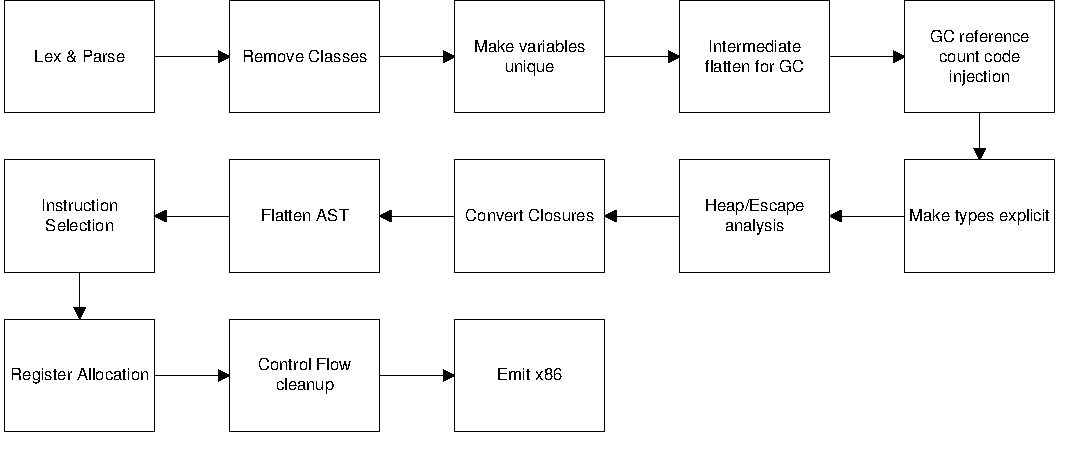
\includegraphics[scale=0.48]{compiler_flow.pdf}
\end{center}
\caption{Compiler Architecture}
\label{fig-comparch}
\end{figure}

\subsubsection{Reference Counting AST Transformation}

Recall that in order to properly maintain reference counts, we need to increment the reference count for an object when a reference is created for it, and decrement the reference count when a reference is destroyed.  References are created by assigning a memory location (which contains an object) to a variable.  References are destroyed when a variable is changed to refer to a different object, or when a variable ceases to exist when a program reaches the end of a given scope.

The most natural way to implement this in our compiler, is to transform our input programs AST such that any assignment to a variable is preceded by a decrement to the reference count for the object the variable refers to, and is succeeded by an increment to the reference count for the newly assigned object.  This is the approach we took, but there are some subtleties with respect to where this operation is placed within the compiler.  Our initial hypothesis was that we could easily add the increment and decrement reference counter operations in the existing ``Flatten AST'' stage.  We quickly realized that because this stage is after type explication, there exist variables which are not \textit{tagged} with a type.  Since we only want to decrement reference counts for \textit{tagged} types\footnote{Actually, we only want to modify reference counts for a subset of tagged types that only includes ``big'' types. However, to simplify our implementation, we transform our AST to always call our increment and decrement runtime functions, but these functions will ignore the primitive types of \texttt{int} and \texttt{boolean}.}, the only option is to put this transformation stage before type explication.  In addition to modifying the AST prior before/after an assignment, the reference counting transformation is also responsible for determining which variables are local to a given scope and decrementing the counts for these references at the end of the given program scope.

\subsubsection{Expressions}
Prior to our explicate phase, complex expressions are not flattened.  This leads to problems where memory is leaked, since no assignments ever occur to temporary objects.  Listing~\ref{lst:simpleleak} shows a program that assigns the result of addition between to lists to the variable \texttt{x}.  The assignment to the variable \texttt{x} results in a corresponding increment reference count on the result of the list addition.  However, the temporary lists, \texttt{[1]} and \texttt{[2]} are leaked if we don't take any additional steps.  To overcome this problem, we introduce a intermediate flattening stage, prior to our reference counting AST transformation.   This results in the corresponding code given in Listing~\ref{lst:flattened} after flattening.  These temporary objects are then deallocated when their corresponding references go out of scope.

\begin{figure}[h!]
\begin{lstlisting}[
language=Python,
frame=none,
xleftmargin=0.2in,
numbers=left,
caption={A simple input program that leaks memory if not flattened.},
captionpos=b,
label=lst:simpleleak
]
x = [1] + [2]
x = 0
print x
\end{lstlisting}
\end{figure}

\begin{figure}[h!]
\begin{lstlisting}[
language=Python,
frame=none,
xleftmargin=0.2in,
numbers=left,
caption={The flattened version of listing \ref{lst:simpleleak}.},
captionpos=b,
label=lst:flattened
]
tmp0 = [1]
tmp1 = [2]
tmp2 = tmp0 + tmp1
x = tmp2
x = 0
print x
\end{lstlisting}
\end{figure}

\subsubsection{Temporary variables}
As a result of introducing the intermediate flattening stage, we introduce additional references to an object which hang around until the end of the given scope.  This is undesirable because it changes the deallocation behavior of the program from the expected behavior.  For original input program in figure~\ref{lst:simpleleak}, the expectation is that when the variable \texttt{x} is assigned the value zero, the reference count for the list object should be decremented to zero and the object deallocated.  However, in the flattened program, this is no longer the case since the \texttt{tmp2} variable continues to reference the object.  The deallocation is therefore delayed until the end of the current scope.  To handle this situation, we keep track of all temporary variables introduced as a result of flattening an expression.  These temporary variables are then assigned a value of zero immediately after the statement containing the expression in which they were introduced.  This will lead to an immediate decrement of the reference count after the reference counting AST transformation.  Figure~\ref{lst:fixflattened} shows the result of the flattening transformation after this change is made.

\begin{figure}[h!]
\begin{lstlisting}[
language=Python,
frame=none,
xleftmargin=0.2in,
numbers=left,
caption={The flattened version of listing \ref{lst:simpleleak} with immediate deallocation of temporary variables.},
captionpos=b,
label=lst:fixflattened
]
tmp0 = [1]
tmp1 = [2]
tmp2 = tmp0 + tmp1
x = tmp2
tmp2 = 0
tmp1 = 0
tmp0 = 0
x = 0
print x
\end{lstlisting}
\end{figure}


\subsubsection{Decrementing reference counts}
As discussed previously, an assignment to a variable should result in a decrement of the reference count for the object referred to by the variable before the assignment.  However, this can't be done when the variable doesn't refer to anything, which is true prior to the initial assignment.  In fact, trying to even access such a variable before it is assigned to can result in undefined results, since there is no guarantee on the contents of the variable (it could be garbage or a value from a previous stack frame).   To prevent a call to \texttt{dec\_ref\_ctr} on a variable before the initial assignment, we initially tried to statically determine when the first assignment occurred.  This approach failed when we realized that for some programs, it is not possible to determine where the initial assignment occurs at compile-time.  Listing~\ref{lst:initialassign} shows an example program where the initial assignment to the variable \texttt{x} cannot be determined statically.  If the input provided by the user evaluates to \texttt{True}, then the initial assignment to $x$ occurs at line 2.  However, if the input evaluates to \texttt{False}, then the initial assignment to \texttt{x} occurs at line 3.  If we transform the input program so that a call is made to decrement the reference count for \texttt{x} immediately prior to the assignment on line 3, then there is the possibility that this will cause the program to crash if the user provides an input that evaluates to \texttt{False}.

To solve this issue, we make a simple change.  We ensure that the value of \texttt{x} is always initialized, by assigning it the value zero at the program scope where it is defined\footnote{Python defines this as the block where a variable is initially assigned to.}.  In our compiler, this is equivalent to a primitive of type \texttt{int}, but this can be any sentinel value that results in a no-op when a call is made to \texttt{dec\_ref\_ctr}.  By ensuring that all local variables are assigned a sentinel value at the beginning of the scope where they are defined, we can safely transform our input program to call \texttt{dec\_ref\_ctr} immediately preceding an assignment, and \texttt{inc\_ref\_ctr} immediately succeeding an assignment.

This solution is somewhat controversial, since it can alter program behavior when the program tries to read from a variable that has not yet been assigned to.  The standard Python interpreter throws a \textit{NameError} in this case, but our compiler will allow such a program to be compiled.  Reading the variable will then result in the sentinel value (zero in our case) being read, instead of the program crashing or having undefined behavior.  A program which used uninitialized (or declared) variables would then have its runtime behavior changed.  Another option to address this issue, is to make it a compile-time error to try and access variable from a conditional block that may have not been previously initialized.  This is similar to a restriction in the Java language.

\begin{figure}[h!]
\begin{lstlisting}[
language=Python,
frame=none,
xleftmargin=0.2in,
numbers=left,
caption={An example program where the initial assignment to \texttt{x} cannot be determined statically.},
captionpos=b,
label=lst:initialassign
]
if input():
    x = [1]
x = [2]
\end{lstlisting}
\end{figure}


\subsubsection{Functions}
The compiler creates temporary variables in a number of situations (namely function calls and as a result of flattened expressions).  These temporary variables need not hang on to their memory reference past the next assignment to the actual result variable.  Any temporary variable is dereferenced immediately at the end of the current scope if it is not the variable being returned.  If it is the return variable we ignore decrementing the reference on this variable, thereby assuring the caller that the object returned is correctly reference counted for its assignment.  If we had decremented the reference counter, due to the immediate nature of garbage collection, we would have been returning a value which did not point to an allocated memory region.

\subsubsection{Addition of Lists}
In the current runtime an entirely new list is created when two lists are added together.  At the assignment level our compiler can determine (due to the flattened structure) that the left-hand-side and the right-hand-side of the addition need their reference counters manipulated, however the assignment from an addition to a list creates an entirely new list which should properly increment the reference counter to all objects in both lists.

\subsubsection{Debugging Integration}
To facilitate debugging in our compiler, we modify the x86 assembly generator to include calls to set up our \texttt{pymem} module and print statistics at the end of the program.

\section{Results}
\label{sec:results}
We evaluated our reference counting implementation for correctness by using the \texttt{valgrind} utility against a simple application that uses a large number of language features.  The program is given below.

\begin{verbatim}
i = 0
list = []
while i !=  10000:
    list = list + [[i]]
    i = i + 1
\end{verbatim}

Without any garbage collection, valgrind reports 

\footnotesize
\begin{verbatim}
LEAK SUMMARY:
   definitely lost: 560,028 bytes in 20,001 blocks
   indirectly lost: 199,004,992 bytes in 20,191 blocks
     possibly lost: 1,375,008 bytes in 19,810 blocks
\end{verbatim}
\normalsize

With our reference counting for the same program

\footnotesize
\begin{verbatim}
LEAK SUMMARY:
   definitely lost: 0 bytes in 0 blocks
   indirectly lost: 0 bytes in 0 blocks
     possibly lost: 0 bytes in 0 blocks
\end{verbatim}
\normalsize


\subsection{Reference counting overhead}

To measure the overhead associated with reference counting, we run 

\subsection{De-allocation latency}

The latency introduced by the \textit{dec\_ref\_ctr} is linear with the number of nodes in the object graph being deallocated.  To illustrate this, the program given in listing~\ref{lst:tree} is run with different inputs, where the input is the height of a 4-ary tree.  The number of nodes in such a tree is given by $\frac{{k}^{\left(h+1\right)}-1}{k-1}$ where $k=4$, and $h$ is the height of tree.  The results are graphed in figure~\ref{fig:treelatency}.  In typical programs, we expect the number of deallocations triggered by any given call to \textit{dec\_ref\_ctr} to be relatively small, but further evaluation of this for real world programs would be needed to prove this hypothesis.

\begin{figure}[h!]
\begin{lstlisting}[
language=Python,
frame=none,
xleftmargin=0.2in,
numbers=left,
caption={An example input program that creates a tree of objects contained in lists.},
captionpos=b,
label=lst:tree
]
def fill(list, i, height):
    if i != height:
        j=0
        while j != 4:
            list[j]=[0,1,2,3]
            fill(list[j], i+1, height)
            j = j + 1
    else:
        0
head=[0,1,2,3]
fill(head, 0, input())
\end{lstlisting}
\end{figure}

\begin{figure}
\normalsize % use normal font size in the figure
% GNUPLOT: LaTeX picture with Postscript
\begingroup
  \makeatletter
  \providecommand\color[2][]{%
    \GenericError{(gnuplot) \space\space\space\@spaces}{%
      Package color not loaded in conjunction with
      terminal option `colourtext'%
    }{See the gnuplot documentation for explanation.%
    }{Either use 'blacktext' in gnuplot or load the package
      color.sty in LaTeX.}%
    \renewcommand\color[2][]{}%
  }%
  \providecommand\includegraphics[2][]{%
    \GenericError{(gnuplot) \space\space\space\@spaces}{%
      Package graphicx or graphics not loaded%
    }{See the gnuplot documentation for explanation.%
    }{The gnuplot epslatex terminal needs graphicx.sty or graphics.sty.}%
    \renewcommand\includegraphics[2][]{}%
  }%
  \providecommand\rotatebox[2]{#2}%
  \@ifundefined{ifGPcolor}{%
    \newif\ifGPcolor
    \GPcolorfalse
  }{}%
  \@ifundefined{ifGPblacktext}{%
    \newif\ifGPblacktext
    \GPblacktexttrue
  }{}%
  % define a \g@addto@macro without @ in the name:
  \let\gplgaddtomacro\g@addto@macro
  % define empty templates for all commands taking text:
  \gdef\gplbacktext{}%
  \gdef\gplfronttext{}%
  \makeatother
  \ifGPblacktext
    % no textcolor at all
    \def\colorrgb#1{}%
    \def\colorgray#1{}%
  \else
    % gray or color?
    \ifGPcolor
      \def\colorrgb#1{\color[rgb]{#1}}%
      \def\colorgray#1{\color[gray]{#1}}%
      \expandafter\def\csname LTw\endcsname{\color{white}}%
      \expandafter\def\csname LTb\endcsname{\color{black}}%
      \expandafter\def\csname LTa\endcsname{\color{black}}%
      \expandafter\def\csname LT0\endcsname{\color[rgb]{1,0,0}}%
      \expandafter\def\csname LT1\endcsname{\color[rgb]{0,1,0}}%
      \expandafter\def\csname LT2\endcsname{\color[rgb]{0,0,1}}%
      \expandafter\def\csname LT3\endcsname{\color[rgb]{1,0,1}}%
      \expandafter\def\csname LT4\endcsname{\color[rgb]{0,1,1}}%
      \expandafter\def\csname LT5\endcsname{\color[rgb]{1,1,0}}%
      \expandafter\def\csname LT6\endcsname{\color[rgb]{0,0,0}}%
      \expandafter\def\csname LT7\endcsname{\color[rgb]{1,0.3,0}}%
      \expandafter\def\csname LT8\endcsname{\color[rgb]{0.5,0.5,0.5}}%
    \else
      % gray
      \def\colorrgb#1{\color{black}}%
      \def\colorgray#1{\color[gray]{#1}}%
      \expandafter\def\csname LTw\endcsname{\color{white}}%
      \expandafter\def\csname LTb\endcsname{\color{black}}%
      \expandafter\def\csname LTa\endcsname{\color{black}}%
      \expandafter\def\csname LT0\endcsname{\color{black}}%
      \expandafter\def\csname LT1\endcsname{\color{black}}%
      \expandafter\def\csname LT2\endcsname{\color{black}}%
      \expandafter\def\csname LT3\endcsname{\color{black}}%
      \expandafter\def\csname LT4\endcsname{\color{black}}%
      \expandafter\def\csname LT5\endcsname{\color{black}}%
      \expandafter\def\csname LT6\endcsname{\color{black}}%
      \expandafter\def\csname LT7\endcsname{\color{black}}%
      \expandafter\def\csname LT8\endcsname{\color{black}}%
    \fi
  \fi
  \setlength{\unitlength}{0.0500bp}%
  \begin{picture}(5040.00,2880.00)%
    \gplgaddtomacro\gplbacktext{%
      \csname LTb\endcsname%
      \put(688,512){\makebox(0,0)[r]{\strut{} 0}}%
      \put(688,784){\makebox(0,0)[r]{\strut{} 0.5}}%
      \put(688,1056){\makebox(0,0)[r]{\strut{} 1}}%
      \put(688,1328){\makebox(0,0)[r]{\strut{} 1.5}}%
      \put(688,1600){\makebox(0,0)[r]{\strut{} 2}}%
      \put(688,1871){\makebox(0,0)[r]{\strut{} 2.5}}%
      \put(688,2143){\makebox(0,0)[r]{\strut{} 3}}%
      \put(688,2415){\makebox(0,0)[r]{\strut{} 3.5}}%
      \put(688,2687){\makebox(0,0)[r]{\strut{} 4}}%
      \put(784,352){\makebox(0,0){\strut{} 0}}%
      \put(1351,352){\makebox(0,0){\strut{} 200}}%
      \put(1917,352){\makebox(0,0){\strut{} 400}}%
      \put(2484,352){\makebox(0,0){\strut{} 600}}%
      \put(3051,352){\makebox(0,0){\strut{} 800}}%
      \put(3618,352){\makebox(0,0){\strut{} 1000}}%
      \put(4184,352){\makebox(0,0){\strut{} 1200}}%
      \put(4751,352){\makebox(0,0){\strut{} 1400}}%
      \put(128,1599){\rotatebox{-270}{\makebox(0,0){\strut{}Latency (seconds)}}}%
      \put(2767,112){\makebox(0,0){\strut{}Number of nodes (in thousands)}}%
    }%
    \gplgaddtomacro\gplfronttext{%
    }%
    \gplbacktext
    \put(0,0){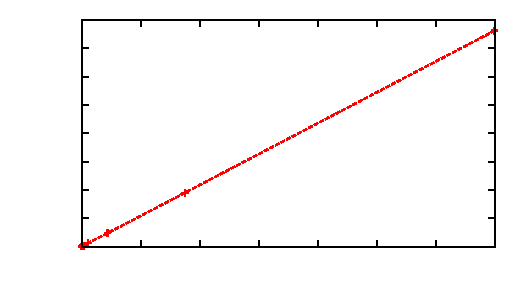
\includegraphics{treelatency}}%
    \gplfronttext
  \end{picture}%
\endgroup

\caption{Latency of \textit{dec\_ref\_ctr} for various size object graphs}
\label{fig:treelatency}
\end{figure}

\section{Future work}
\label{sec:future}

Optimizations.

\section{Conclusions}
\label{sec:conclusion}

\subsection{Disadvantages}

\subsection{Advantages}

%\appendix
%\section{Appendix Title}
% This is the text of the appendix, if you need one.

\acks

We would like to thank Jeremy Siek and Evan Chang for the course notes from which the compiler design is derived.

% We recommend abbrvnat bibliography style.

\bibliographystyle{abbrvnat}

% The bibliography should be embedded for final submission.

\begin{thebibliography}{}
\softraggedright

\bibitem{boehm}
Hans-J. Boehm. 2004. The space cost of lazy reference counting. In Proceedings of the 31st ACM SIGPLAN-SIGACT symposium on Principles of programming languages (POPL '04). ACM, New York, NY, USA, 210-219. DOI=10.1145/964001.964019 

\bibitem{joisha}
Pramod G. Joisha. 2006. Compiler optimizations for nondeferred reference: counting garbage collection. In Proceedings of the 5th international symposium on Memory management (ISMM '06). ACM, New York, NY, USA, 150-161. DOI=10.1145/1133956.1133976

\bibitem{blackburn}
Stephen M. Blackburn and Kathryn S. McKinley. 2003. Ulterior reference counting: fast garbage collection without a long wait. In Proceedings of the 18th annual ACM SIGPLAN conference on Object-oriented programing, systems, languages, and applications (OOPSLA '03). ACM, New York, NY, USA, 344-358. DOI=10.1145/949305.949336

\bibitem{lin}
Chin-Yang Lin and Ting-Wei Hou. 2010. An efficient approach to cyclic reference counting based on a coarse-grained search. Inf. Process. Lett. 111, 1 (December 2010), 1-10. DOI=10.1016/j.ipl.2010.10.004 

\bibitem{trancon}
Baltasar Trancón y Widemann. 2008. A reference-counting garbage collection algorithmfor cyclical functional programming. In Proceedings of the 7th international symposium on Memory management (ISMM '08). ACM, New York, NY, USA, 71-80. DOI=10.1145/1375634.1375645 

\bibitem{joao}
José A. Joao, Onur Mutlu, and Yale N. Patt. 2009. Flexible reference-counting-based hardware acceleration for garbage collection. In Proceedings of the 36th annual international symposium on Computer architecture (ISCA '09). ACM, New York, NY, USA, 418-428. DOI=10.1145/1555754.1555806

\bibitem{hertz}
Matthew Hertz and Emery D. Berger. 2005. Quantifying the performance of garbage collection vs. explicit memory management. In Proceedings of the 20th annual ACM SIGPLAN conference on Object-oriented programming, systems, languages, and applications (OOPSLA '05). ACM, New York, NY, USA, 313-326. DOI=10.1145/1094811.1094836  

\bibitem{levanoni}
Yossi Levanoni and Erez Petrank. 2006. An on-the-fly reference-counting garbage collector for java. ACM Trans. Program. Lang. Syst. 28, 1 (January 2006), 1-69. DOI=10.1145/1111596.1111597 

\bibitem{ritzaou}
Tobias Ritzau. 1999.  Real-Time Reference Counting in RT-Java

\bibitem{siek}
Jeremy G. Siek. 2011.  A Problem Course in Compilation: From Python to x86 Assembly

\end{thebibliography}

\end{document}
